%!TEX program = xelatex
\documentclass[cn,hazy,pku,12pt,normal,math=newtx,cite=super]{elegantnote}
\title{磁化率的测定}

\author{刘松瑞 \quad 2100011819 \\ 组号:24 \quad 组内编号:5}
\institute{化学与分子工程学院}

\expdate{\zhdate{2023/12/7}}
\temperature{20.6 \si{^{\circ}C}}
\pressure{99.70 \si{kPa}}

\usepackage{gensymb}
\usepackage{array}
\usepackage{subfigure}
\usepackage[fontset=windows]{ctex}
\usepackage{graphicx}
\usepackage{float}
\usepackage{caption}
\usepackage{multirow}
%\usepackage{subfig}
%\usepackage{float}
\begin{document}

\maketitle

\abstracts{
    本实验采用 Guoy 磁天平法,并以莫尔盐为标准样品,在室温 21.9 °C 下,测得了计算得到硫酸铜的摩尔磁化率 $\rm 1.93 \pm 0.04 \times 10^{-8} m^3\ \cdot mol^{-1}$
,亚铁氰化钾的摩尔磁化率 $\rm - 0.1 \pm 0.1 \times 10^{-8} m^3\ \cdot mol^{-1}$
,样品的比磁化率 $\rm 1.75 \pm 0.04 \times 10^{-7} m^3\ \cdot kg^{-1}$ 。计算分析得到硫酸铜的分子磁矩为1.89 $\mu B$,
有一个不成对电子;亚铁氰化钾为反磁性物质,没有不成对电子。实验的主要误差来自于质量变化的测量误差。
}
\keywords{
    Guoy 磁天平法\quad 硫酸铜\quad 磁化率 \quad 亚铁氰化钾
}

\newpage


\section{引言}

\subsection{实验目的、原理与方法}
\subsubsection[short]{实验目的}
\begin{enumerate}
    \item 掌握 Guoy 磁天平法测定磁化率的原理与方法。
    \item 利用 Guoy 磁天平测定几种固体物质的磁化率,计算其摩尔磁化率,并估算离子的不成对数。
\end{enumerate}

\subsubsection[short]{实验原理与方法}
实验原理与方法详见预习报告图~\ref{1}。 \cite{pcl2002}

\begin{figure}[htbp]
    \centering
    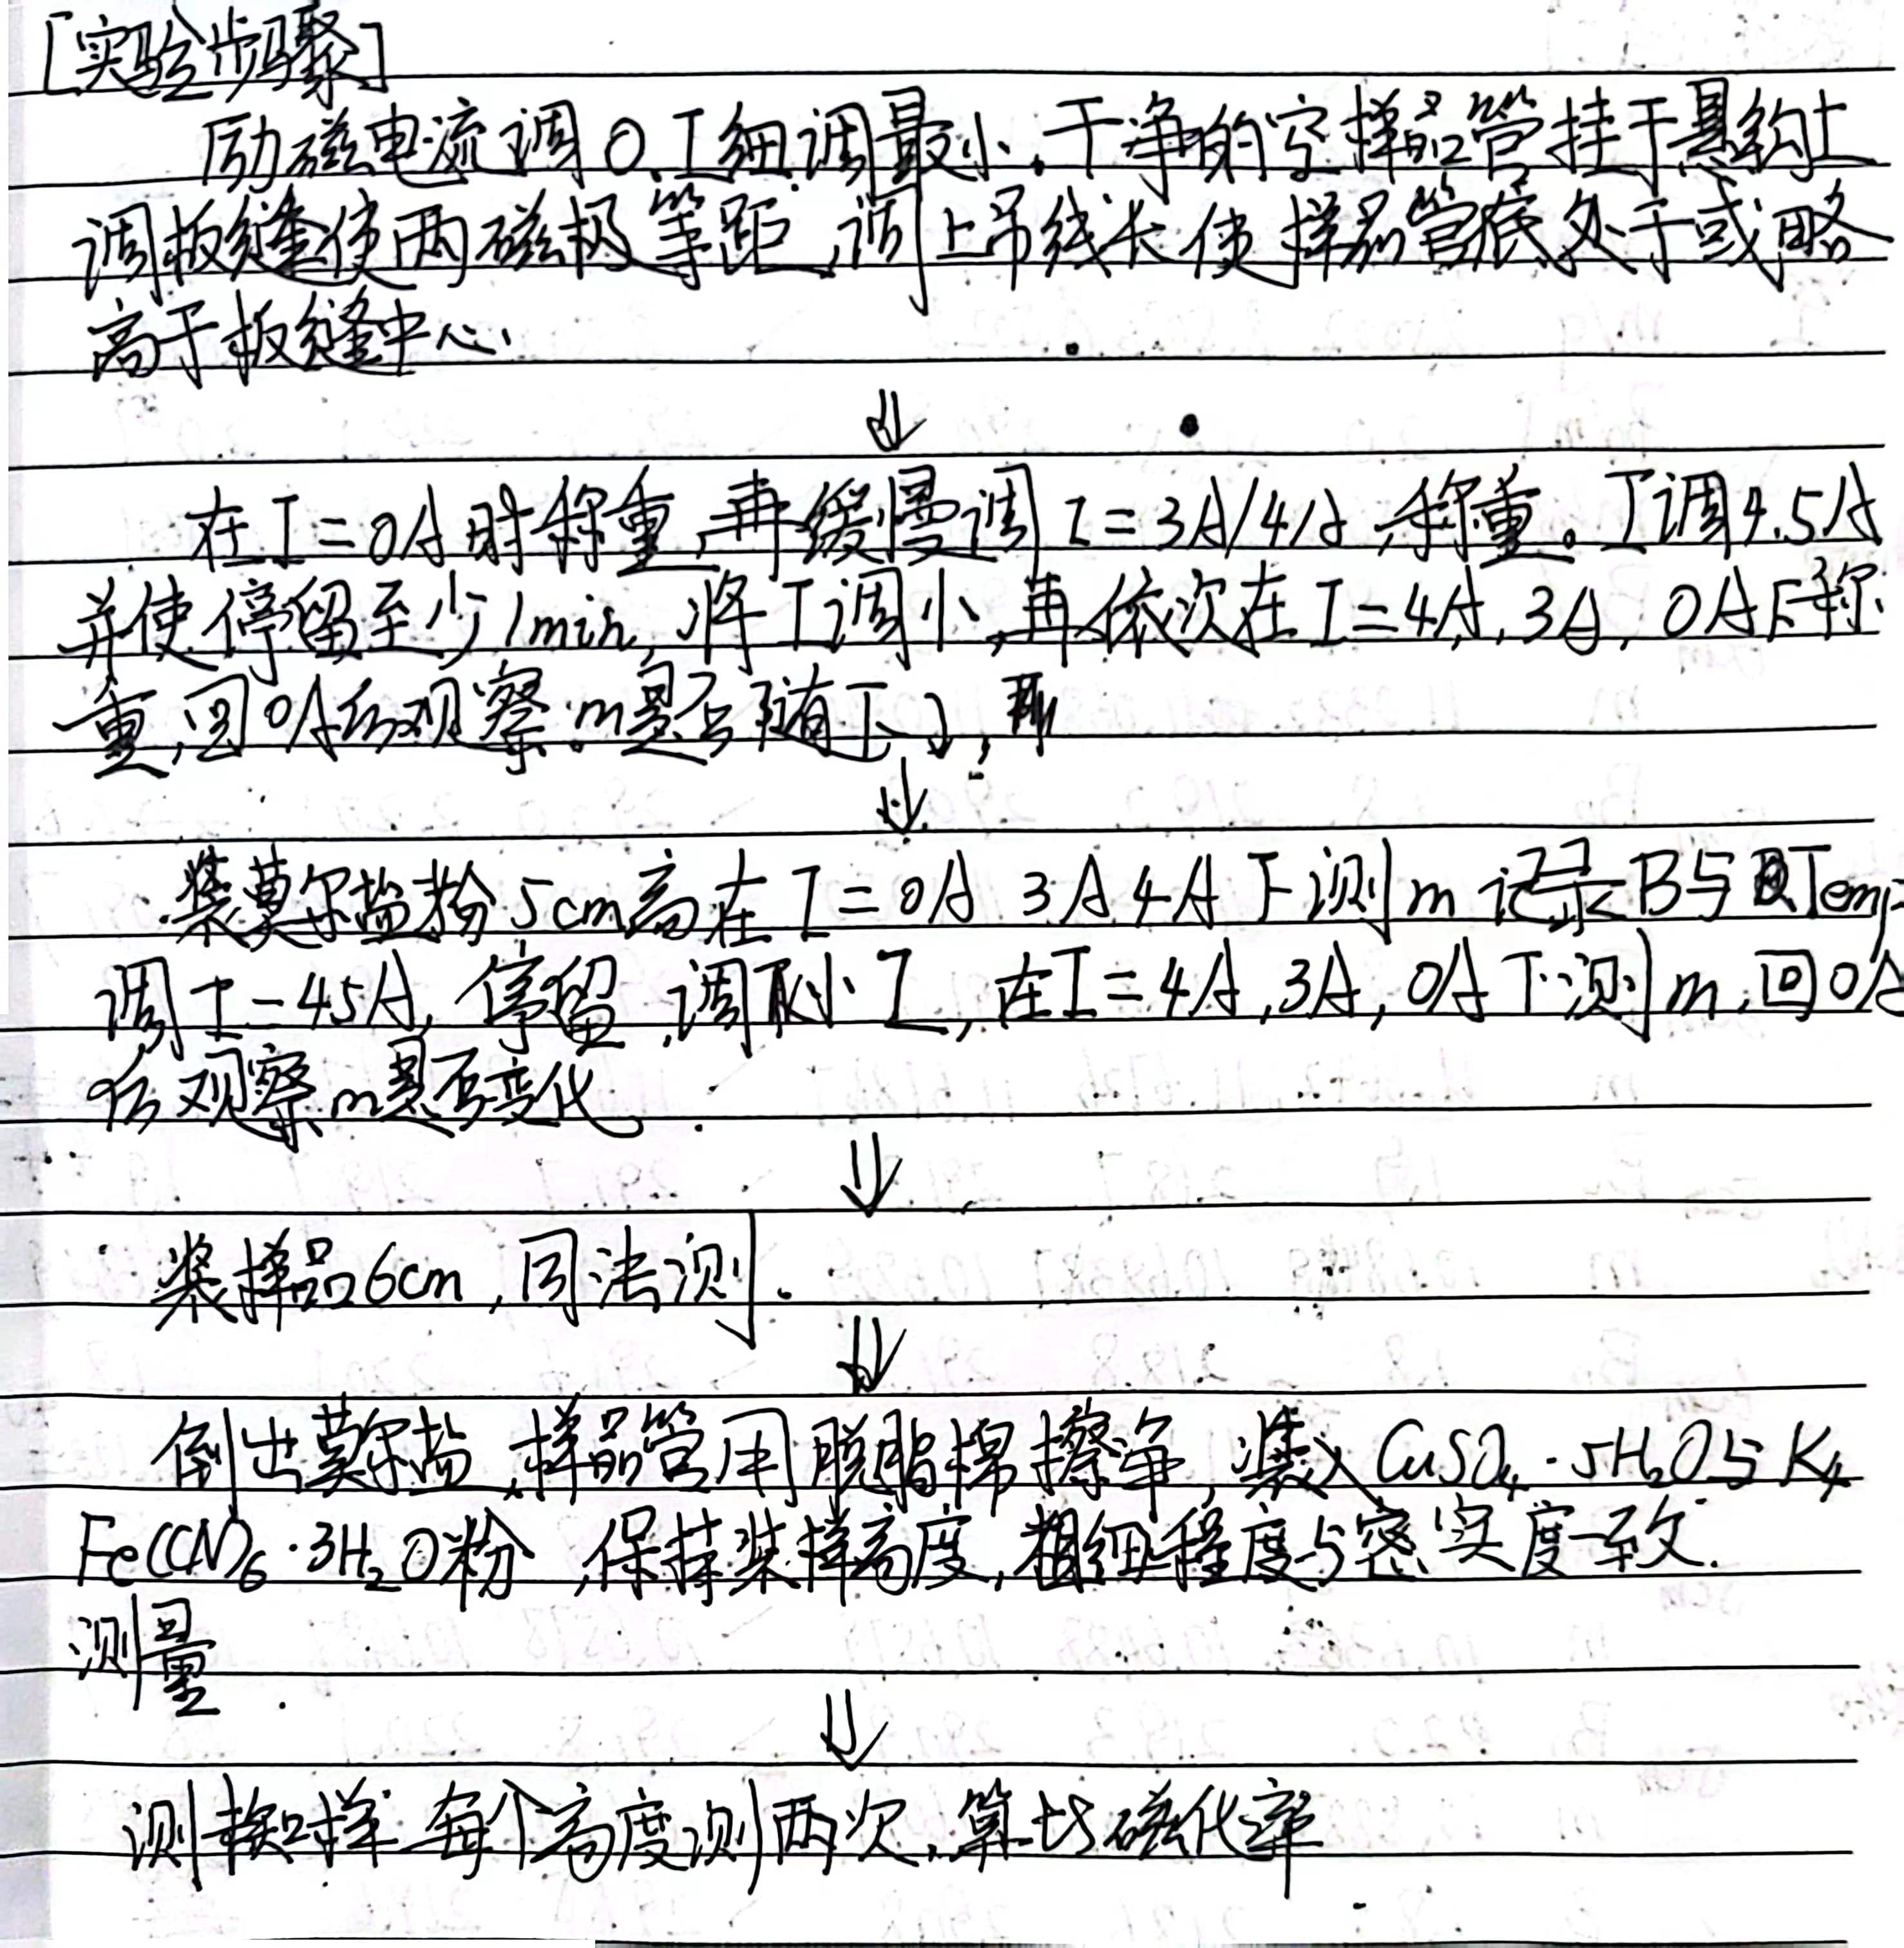
\includegraphics[width = .70\textwidth]{image/yxbg_1.jpg}
    \caption{实验的目的与原理}\label{1}
\end{figure}

\section{实验部分}

\subsection{实验步骤}
实验步骤详见预习报告图~\ref{2}。

\begin{figure}[htbp]
    \centering
    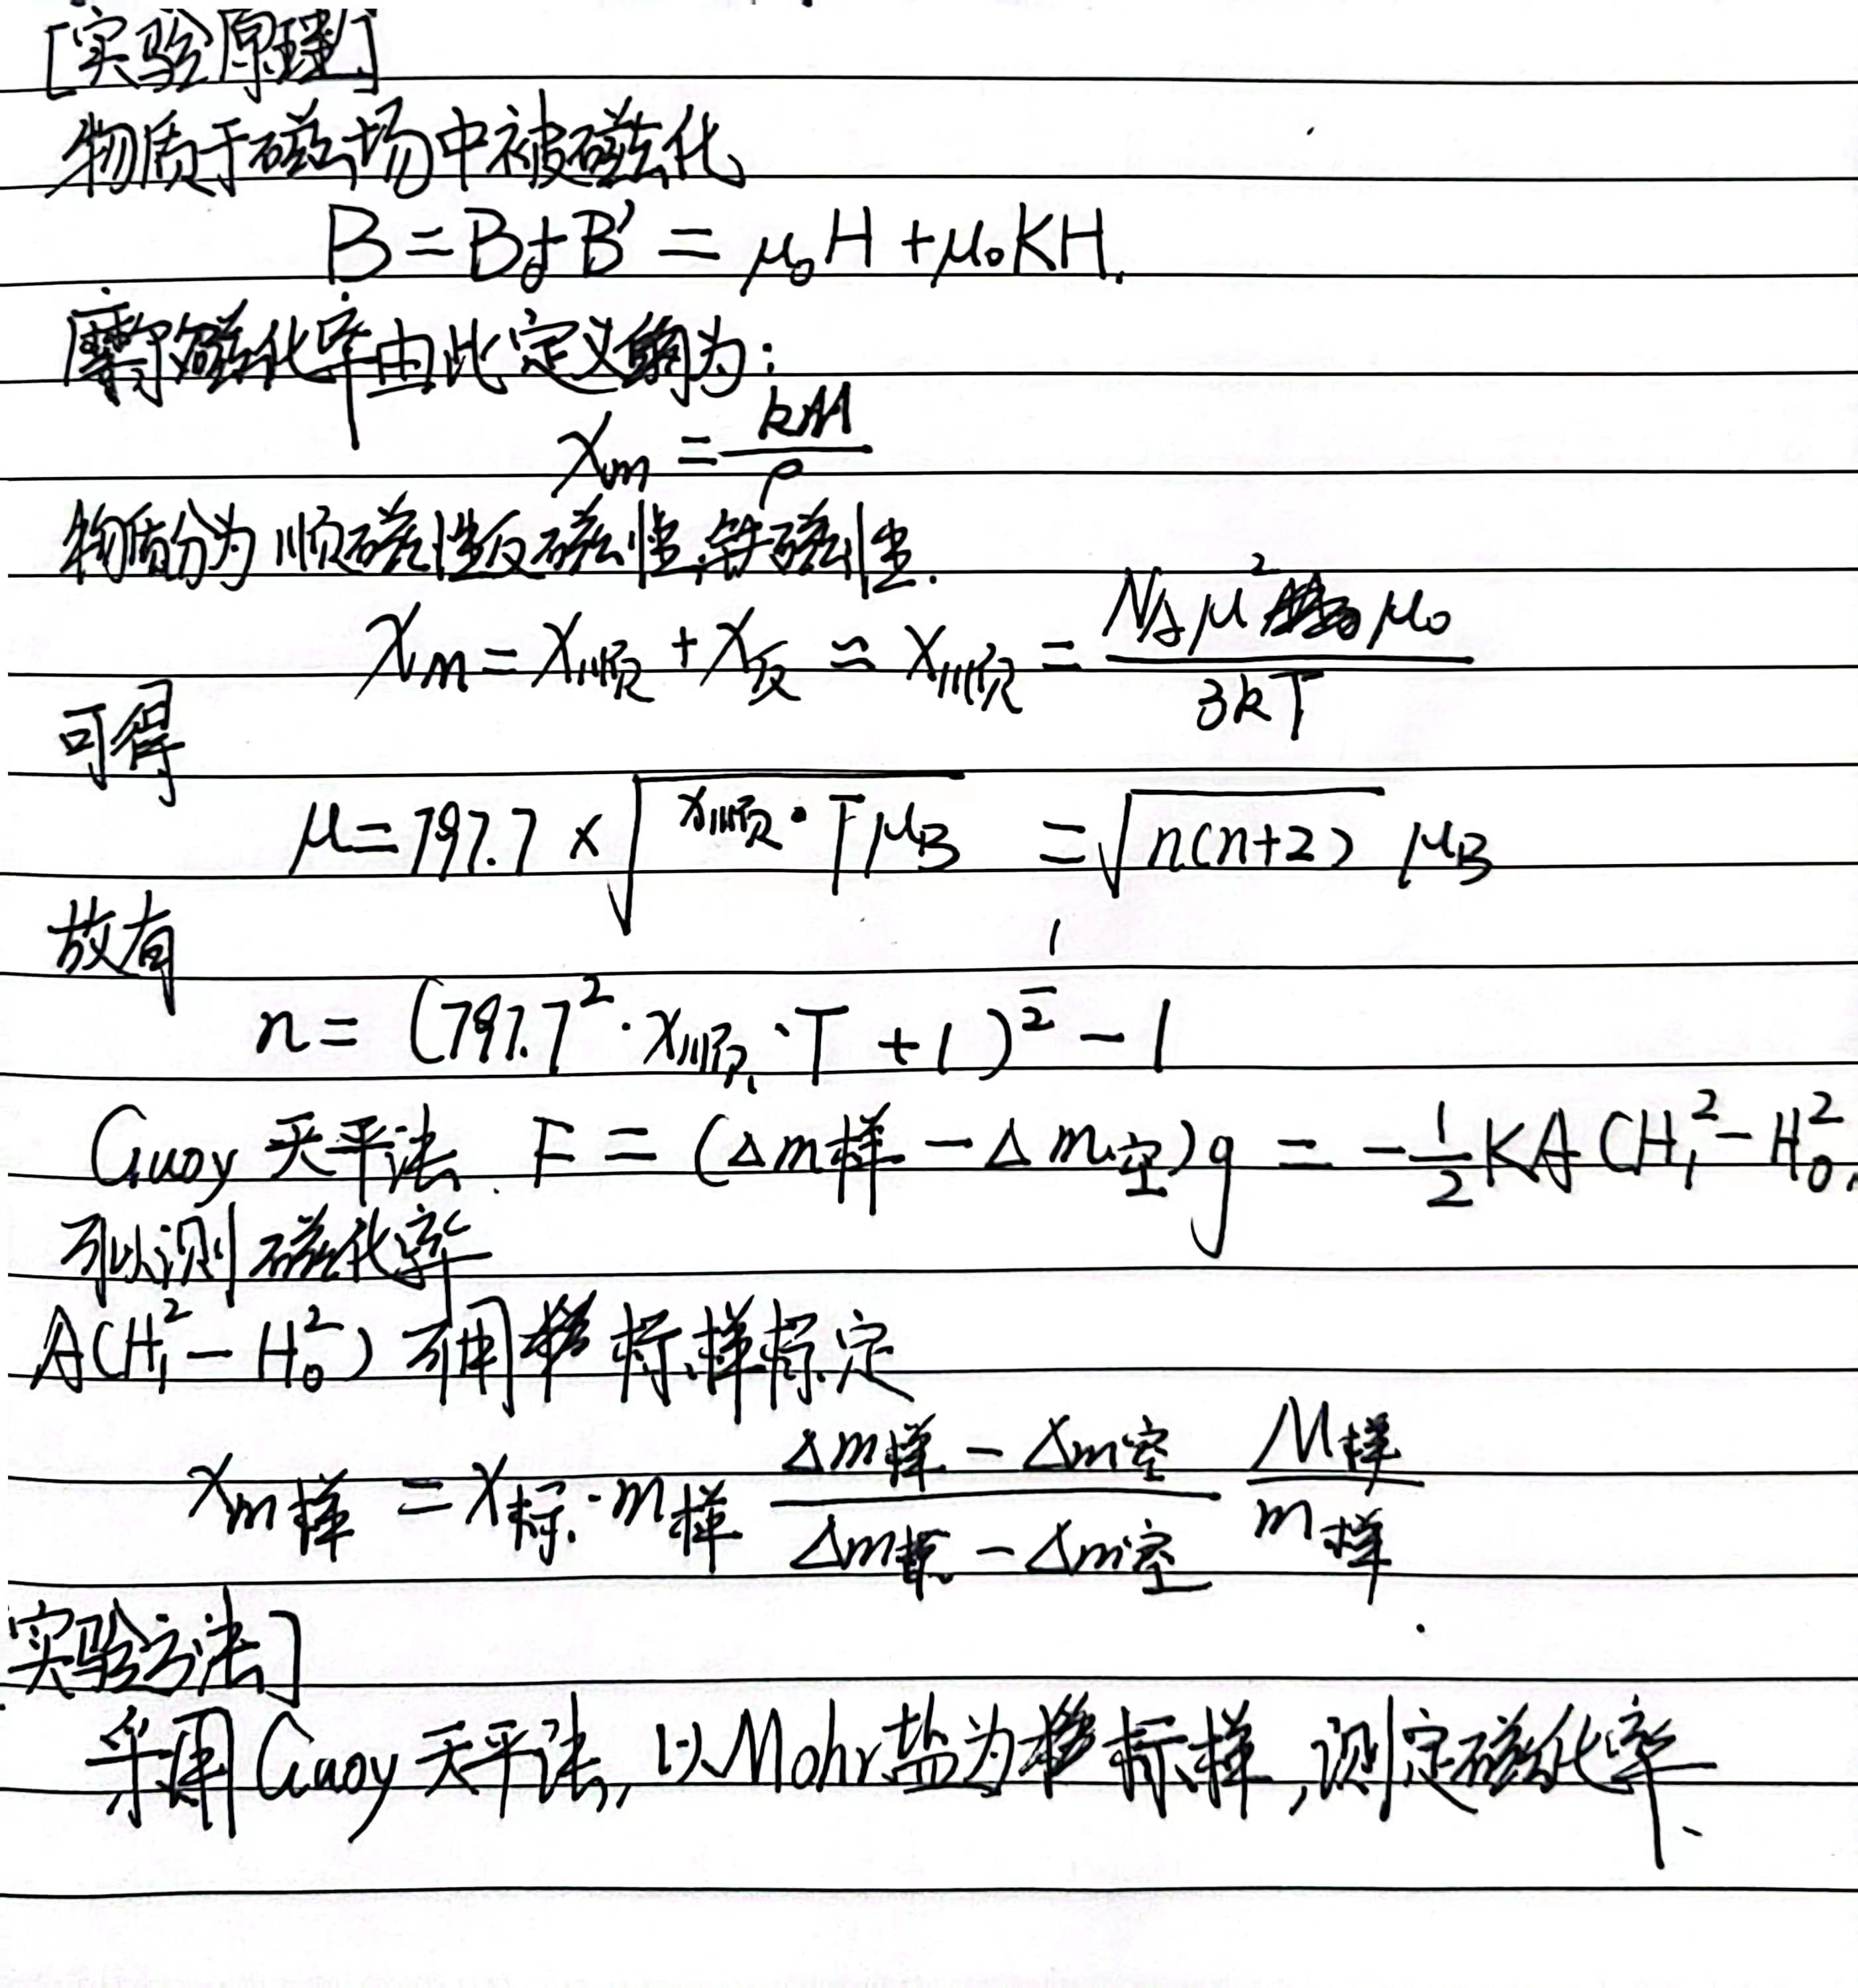
\includegraphics[width = .70\textwidth]{image/yxbg_2.jpg}
    \caption{实验的目的与原理}\label{2}
\end{figure}

\subsection{仪器与药品}

\begin{enumerate} %有序列表
    \item 试剂 \\   莫尔盐 (AR),$\rm CuSO_4 \cdot 5H_2O(AR),\  K_4Fe(CN)_6 \cdot 3H_2O(AR)$,未知样;
    \item 仪器 \\   磁天平(配电子天平),研钵,试管。
\end{enumerate}

\section{实验现象与数据处理}
\subsection[short]{数据记录}
实验温度为 $\rm T = 20.6\ \degree C = 293.15\ K$ ,实验中物质的质量与磁场强度如表\ref{01}所示,
并计算不同励磁电流下质量变化如表 \ref{02} 。

% Please add the following required packages to your document preamble:
% \usepackage{multirow}
\begin{table}[h]
    \centering
    \caption{实验过程中的磁场强度与各物质的质量}
    \label{01}
    \begin{tabular}{cccccccccc}
    \hline
    \multicolumn{2}{c}{励磁电流/A}                     &       & 0       & 3       & 4       & 4.5 & 4       & 3       & 0       \\ \hline
    \multicolumn{2}{c}{\multirow{2}{*}{空管}}        & $B_0$ & 1.9     & 218.8   & 291.0     & /   & 291.4   & 220.1   & 2.0       \\
    \multicolumn{2}{c}{}                           & m     & 8.5037  & 8.5026  & 8.5020   & /   & 8.5020   & 8.5029  & 8.5037  \\\hline
    \multirow{4}{*}{莫尔盐} & \multirow{2}{*}{5 cm} & $B_0$ & 2.0       & 218.5   & 290.9   & /   & 291.4   & 220.1   & 2.0       \\
                           &                       & m     & 10.5620  & 10.5950  & 10.6195 & /   & 10.6196 & 10.5956 & 10.5631 \\
                           & \multirow{2}{*}{6 cm} & $B_0$ & 1.9     & 219.0     & 291.3   & /   & 291.9   & 219.5   & 2.0       \\
                           &                       & m     & 11.0332 & 11.0681 & 11.0944 & /   & 11.0950  & 11.0683 & 11.0337 \\\hline
    \multirow{4}{*}{硫酸铜} & \multirow{2}{*}{5 cm} & $B_0$ & 1.8     & 219.2   & 290.8   & /   & 292     & 220.1   & 2.0       \\
                           &                       & m     & 11.0916 & 11.0995 & 11.1050  & /   & 11.1054 & 11.0995 & 11.0917 \\
                           & \multirow{2}{*}{6 cm} & $B_0$ & 1.8     & 218.8   & 291.0     & /   & 291.8   & 219.6   & 1.8     \\
                           &                       & m     & 11.6642 & 11.6726 & 11.6787 & /   & 11.6789 & 11.6727 & 11.6644 \\\hline
    \multirow{4}{*}{亚铁氰化钾} & \multirow{2}{*}{5 cm} & $B_0$ & 1.9     & 218.7   & 291.3   & /   & 291.7   & 219.7   & 1.9     \\
                           &                       & m     & 10.6849 & 10.6837 & 10.6829 & /   & 10.6827 & 10.6838 & 10.6849 \\
                           & \multirow{2}{*}{6 cm} & $B_0$ & 1.8     & 218.8   & 291.3   & /   & 291.6   & 220.1   & 1.8     \\
                           &                       & m     & 11.1839 & 11.1828 & 11.1815 & /   & 11.1818 & 11.1826 & 11.1840  \\\hline
    \multirow{8}{*}{样品}    & \multirow{2}{*}{5 cm} & $B_0$ & 1.8     & 219.3   & 291.1   & /   & 291.8   & 220.0     & 1.8     \\
                           &                       & m     & 10.6367 & 10.6488 & 10.6579 & /   & 10.6578 & 10.6488 & 10.6367 \\
                           & \multirow{2}{*}{5 cm} & $B_0$ & 2.0       & 219.3   & 290.9   & /   & 291.8   & 220.1   & 1.8     \\
                           &                       & m     & 10.5887 & 10.6010  & 10.6099 & /   & 10.6102 & 10.6012 & 10.5888 \\
                           & \multirow{2}{*}{6 cm} & $B_0$ & 1.8     & 218.6   & 290.8   & /   & 291.5   & 219.6   & 2.0       \\
                           &                       & m     & 11.1541 & 11.1675 & 11.1777 & /   & 11.1778 & 11.1678 & 11.1545 \\
                           & \multirow{2}{*}{6 cm} & $B_0$ & 1.8     & 219.5   & 292.0     & /   & 292.0     & 220.0     & 1.8     \\
                           &                       & m     & 11.1658 & 11.1791 & 11.1902 & /   & 11.1901 & 11.1800   & 11.1660  \\ \hline
    \end{tabular}
\end{table}

% Please add the following required packages to your document preamble:
% \usepackage{multirow}
\begin{table}[h]
    \centering
    \caption{不同条件下样品的质量变化}
    \label{02}
    \begin{tabular}{clcccccc}
    \hline
                           & \multicolumn{1}{c}{} & $m/g$   & $\Delta m_{3A}$/g & $\Delta m_{4A}$/g & $\Delta m_{4A}$/g & $\Delta m_{3A}$/g & $\Delta m_{0A}$/g \\ \hline
    \multicolumn{2}{c}{空管}      & 8.5037  & -0.0011&	-0.0017	&-0.0017	&-0.0008&	0.0000 \\ \hline
    \multirow{2}{*}{莫尔盐} & 5 cm & 10.5620 & 0.0330  & 0.0575  & 0.0576  & 0.0336  & 0.0011 \\
                         & 6 cm & 11.0332 & 0.0349  & 0.0612  & 0.0618  & 0.0351  & 0.0005 \\ \hline
    \multirow{2}{*}{硫酸铜} & 5 cm & 11.0916 & 0.0079  & 0.0134  & 0.0138  & 0.0079  & 0.0001 \\
                         & 6 cm & 11.6642 & 0.0084  & 0.0145  & 0.0147  & 0.0085  & 0.0002 \\ \hline
    \multirow{2}{*}{亚铁氰化钾} & 5 cm                 & 10.6849 & -0.0012           & -0.0020           & -0.0022           & -0.0011           & 0.0000            \\
                         & 6 cm & 11.1839 & -0.0011 & -0.0024 & -0.0021 & -0.0013 & 0.0001 \\ \hline
    \multirow{4}{*}{样品}  & 5 cm & 10.6367 & 0.0121  & 0.0212  & 0.0211  & 0.0121  & 0.0000 \\
                         & 5 cm & 10.5887 & 0.0123  & 0.0212  & 0.0215  & 0.0125  & 0.0001 \\
                         & 6 cm & 11.1541 & 0.0134  & 0.0236  & 0.0237  & 0.0137  & 0.0004 \\
                         & 6 cm & 11.1658 & 0.0133  & 0.0244  & 0.0243  & 0.0142  & 0.0002 \\ \hline
    \end{tabular}
\end{table}
\subsection[short]{磁化率的计算}
由公式,
$$
\chi_{Mohr} = \frac{4 \pi \cdot 9.500 \times 10^{-6}}{T+1} = 4.584 \times 10^{-7} m^3\cdot kg^{-1}
$$

计算得到,莫尔盐的磁化率为 $ 4.584 \times 10^{-7}\ m^3\cdot kg^{-1} $
,通过以下公式可以计算比磁化率
$$
\chi^,_{m_{sample}} = \chi_{m_{standard}}\frac{\Delta m_{sample} - \Delta m_{blank}}{ \Delta m_{standard} - \Delta m_{blank}}\times \frac{m_{standard}}{m_{sample}} 
$$

样品的磁化率可以由下计算得到
$$
\chi_{m_{sample}} = \chi^,_{m_{sample}} \times M_{sample}
$$

计算得到硫酸铜、亚铁氰化钾在不同条件下的摩尔磁化率如下表 \ref{03} 所示,由于不知道样品的
摩尔质量,因此只能计算得到比磁化率如下表 \ref{04} 所示

% Please add the following required packages to your document preamble:
% \usepackage{multirow}
\begin{table}[h]
    \centering
    \caption{硫酸铜、亚铁氰化钾在不同条件下的摩尔磁化率}
    \label{03}
    \begin{tabular}{ccccc}
    \hline
    样品                     & 样品高度                  & 励磁电流 & \multicolumn{2}{c}{$\chi$/$10^{-8} m^3   \cdot mol^{-1}$} \\ \hline
    \multirow{4}{*}{硫酸铜} & \multirow{2}{*}{5 cm} & 3A       & 1.90          & 1.86                        \\
                           &                       & 4A       & 1.90          & 1.96                        \\
                           & \multirow{2}{*}{6 cm} & 3A       & 1.94          & 1.95                        \\
                           &                       & 4A       & 1.96          & 1.97                        \\ \hline
    \multirow{4}{*}{亚铁氰化钾} & \multirow{2}{*}{5 cm} & 3A   & -0.03         & -0.10                       \\
                           &                       & 4A       & -0.06         & -0.10                       \\
                           & \multirow{2}{*}{6 cm} & 3A       & 0.00          & -0.16                       \\
                           &                       & 4A       & -0.13         & -0.07                       \\ \hline
    \end{tabular}
    \end{table}

% Please add the following required packages to your document preamble:
% \usepackage{multirow}
\begin{table}[h]
    \centering
    \caption{未知样的比磁化率
    }
    \label{04}
    \begin{tabular}{ccccc}
    \hline
     &
      $\chi^,_{3A}$/$\rm 10^{-7} m^3 \cdot   kg^{-1}$ &
      $\chi^,_{4A}$/$\rm 10^{-7} m^3 \cdot   kg^{-1}$ &
      $\chi^,_{4A}$/$\rm 10^{-7} m^3 \cdot   kg^{-1}$ &
      $\chi^,_{3A}$/$\rm 10^{-7} m^3 \cdot   kg^{-1}$ \\ \hline
    5 cm & 1.71 & 1.71 & 1.70 & 1.66 \\
    5 cm & 1.78 & 1.75 & 1.77 & 1.75 \\
    6 cm & 1.76 & 1.76 & 1.75 & 1.77 \\
    6 cm & 1.74 & 1.81 & 1.78 & 1.82 \\ \hline
    \end{tabular}
\end{table}

观察各个样品的摩尔磁化率与比磁化率,硫酸铜与未知样的平行度较好,
极差均在 
0.1$\rm \times 10^{-8} m^3 \cdot mol^{-1}$
与 0.1$\rm \times 10^{-7} m^3 \cdot kg^{-1}$以内

由于下行时样品会存在剩磁现象,因此只取硫酸铜与亚铁氰化钾的上行部分
求平均值,得:
$$
\rm \chi_{CuSO_4} = 1.93 \times 10^{-8} m^3\ \cdot mol^{-1}
$$
$$
\rm \chi_{KFe(CN)_6} = -0.06 \times 10^{-8} m^3\ \cdot mol^{-1}
$$

同样地我们对样品的比磁化率
求平均值,得:
$$
\rm\chi^,_{sample} = 1.75 \times 10^{-8} m^3\ \cdot kg^{-1}
$$
\subsection[short]{分子磁矩与单电子数的计算}

由公式,
$$
\rm \mu = 797.7 \times \sqrt{\frac{\chi_p}{m^3 \cdot mol^{-1}} \frac{T}{K}} \mu_B
$$

由表 \ref{03} 的数据,可以计算得到硫酸铜的分子磁矩如下表 \ref{05}。

\begin{table}[h]
    \centering
    \caption{硫酸铜在不同条件下的分子磁矩}
    \label{05}
    \begin{tabular}{ccc}\hline
         & $\mu_{3A}/\mu_B$ & $\mu_{4A}/\mu_B$ \\\hline
    5 cm & 1.88     & 1.88     \\
    6 cm & 1.90     & 1.91    \\\hline
    \end{tabular}
\end{table}

可以得到硫酸铜的平均磁矩为 1.89 $\mu_B$。

若将亚铁氰化钾的数据代入公式中,根号下为负数,没有意义。这是由于亚铁氰化钾是一种反磁性物质,
测得的 $\chi_m$ 为反磁性的磁矩 $\chi_d$,因此亚铁氰化钾的分子磁矩是 0 ,无单电子。

又由于
$$
\mu = \sqrt{n(n+2)}
$$

可以计算硫酸铜的单电子数如下表 \ref{06} 所示。

\begin{table}[h]
    \centering
    \caption{硫酸铜在不同条件下的单电子数}
    \label{06}
    \begin{tabular}{ccc}\hline
         & $n_{3A}$ & $n_{4A}$ \\\hline
    5 cm & 1.13     & 1.13     \\
    6 cm & 1.15     & 1.16    \\\hline
    \end{tabular}
\end{table}

可以得到硫酸铜的测量的平均单电子数为 1.14 ,因此硫酸铜分子的单电子数为 1 个,这与硫酸铜
的实际分子结构相吻合。

由于未知样的摩尔质量未知,因此无法进行分子磁矩与不成对电子数的计算。

\subsection[short]{误差计算}

本次实验误差的主要来源为磁场强度的误差,天平称量的误差。
查阅 \cite{CRC}文献,可以得到
$$
\rm \chi_{CuSO_4}^o = 1.835 \times 10^{-8} m^3\ \cdot mol^{-1}
$$

虽然实验所用的天平较为精准,为万分之一分析天平,但是由于实验中样品在磁场下的质量变化很小,
称量误差仍然较大,称量误差为 $\pm 0.1 mg$。
$$
\chi_{m_{sample}} = \chi_{m_{standard}}\frac{\Delta m_{sample} - \Delta m_{blank}}{ \Delta m_{standard} - \Delta m_{blank}}\times \frac{m_{standard} M_{sample}}{m_{sample}} 
$$
$$
\sigma_{m_{standard}} = \sqrt{2} \sigma_{m} =  0.1 mg
$$
$$
\sigma_{m_{sample}} = \sqrt{2} \sigma_{m} = 0.1 mg
$$
$$
\sigma_{\Delta m_{sample} - \Delta m_{blank}}=\sigma_{\Delta m_{standard} - \Delta m_{blank}} =  \sqrt{4} \sigma_{m} = 0.2 mg
$$

\begin{equation*}
    \begin{aligned}
         \sigma_\chi &= \chi_{m_{sample}} \sqrt{(\frac{\sigma_{m_{standard}}}{m_{standard}})^2+(\frac{\sigma_{m_{sample}}}{m_{sample}})^2+(\frac{\sigma_{\Delta m_{sample} - \Delta m_{blank}}}{\Delta m_{sample} - \Delta m_{blank}})^2+(\frac{\sigma_{\Delta m_{standard} - \Delta m_{blank}}}{\Delta m_{standard} - \Delta m_{blank}})^2} \\
                    &= 0.04 \times 10^{-8} m^3\ \cdot mol^{-1}
    \end{aligned}
\end{equation*}

$$
\rm \chi_{CuSO_4} = 1.93 \pm 0.04 \times 10^{-8} m^3\ \cdot mol^{-1}
$$
计算得到硫酸铜的摩尔磁化率 $\rm 1.93 \pm 0.04 \times 10^{-8} m^3\ \cdot mol^{-1}$
 ,然后同理得到亚铁氰化钾的摩尔磁化率 $\rm - 0.1 \pm 0.1 \times 10^{-8} m^3\ \cdot mol^{-1}$
,样品的比磁化率 $\rm 1.75 \pm 0.04 \times 10^{-7} m^3\ \cdot kg^{-1}$ 。
可以看出,亚铁氰化钾的摩尔磁化率测量误差较大,这是因为亚铁氰化钾的摩尔磁化率很低,测量时
质量变化很小,导致质量变化的相对误差很大。

可能的误差来源有:
\begin{enumerate}
    \item 每次装样的时候都要求粗细紧密程度一致,但实际操作误差很大。
    \item 由于磁滞效应,在励磁电流减小的过程中,读数可能会偏大。
    \item 电流调至相同值时,磁场强度存在波动。
    \item 样品管每次悬挂的高度不一定相同。
\end{enumerate}


\section{实验结果与讨论}
\subsection{结论}

本实验采用 Guoy 磁天平法,并以莫尔盐为标准样品,在室温 21.9 °C 下,测得了计算得到硫酸铜的摩尔磁化率 $\rm 1.93 \pm 0.04 \times 10^{-8} m^3\ \cdot mol^{-1}$
,亚铁氰化钾的摩尔磁化率 $\rm - 0.1 \pm 0.1 \times 10^{-8} m^3\ \cdot mol^{-1}$
,样品的比磁化率 $\rm 1.75 \pm 0.04 \times 10^{-7} m^3\ \cdot kg^{-1}$ 。计算分析得到硫酸铜的分子磁矩为1.89 $\mu B$,
有一个不成对电子;亚铁氰化钾为反磁性物质,没有不成对电子。实验的主要误差来自于质量变化的测量误差。

\newpage

\section{附录}
\begin{figure}[htbp]
    \centering
    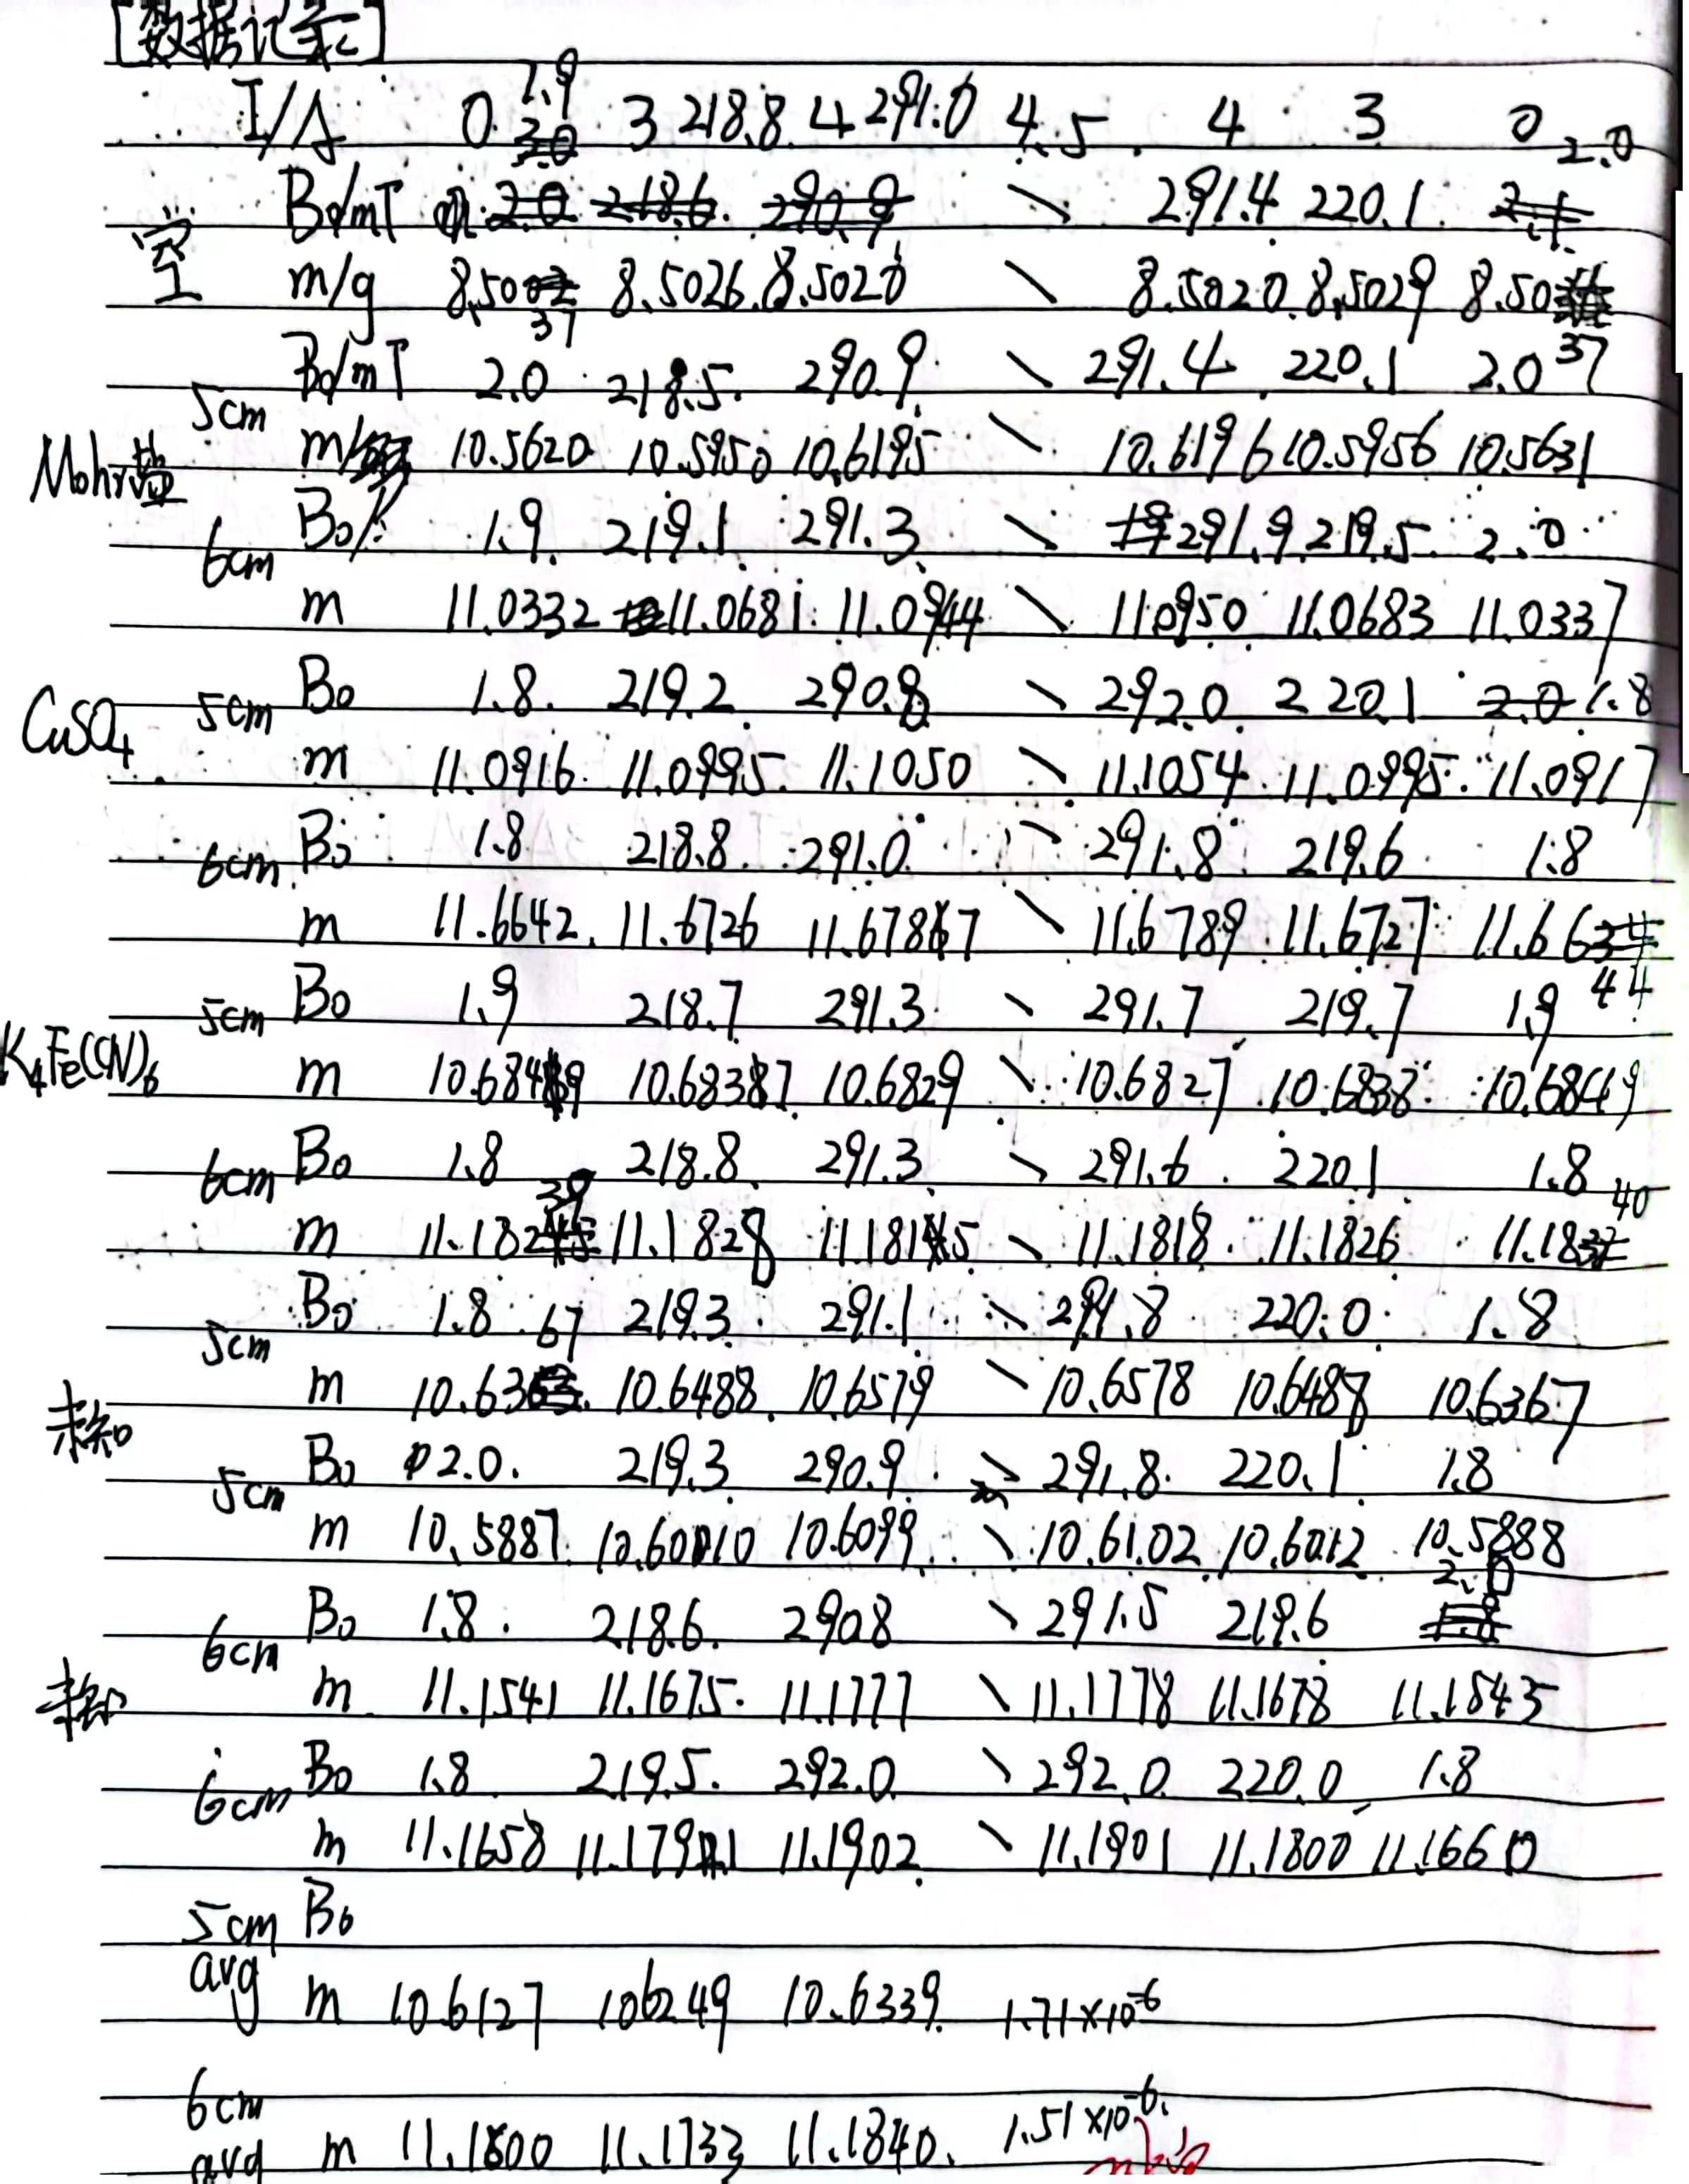
\includegraphics[width = .70\textwidth]{image/sysj.jpg}
    \caption{数据记录图片}\label{3}
\end{figure}
\nocite{*}

\newpage
\bibliography{reference}
\end{document}
